\subsection{Quick starter}

After installation, it is easy to explore the user interfaces automatically
generated by \alida using the shipped demo operators.

The generic graphical user interface may be invoked using the application
\icode{ALDOpRunnerGUI} in the package
\icode{de.unihalle.informatik.Alida.tools}.
It may be started from your favorite IDE or from the command line by
\vspace*{0.5cm}
\begin{code}
        java de.unihalle.informatik.Alida.tools.ALDOpRunnerGUI
\end{code}

\vspace*{-0.25cm}
as soon as the \icode{CLASSPATH} is set correctly, i.e., it needs to include
Alida's jar archive and all its dependencies. Running the above command will
bring up a window displaying a package tree of all available operators, which
are mainly given by the set of demo operators shipped with \alida (see
Fig.~\ref{fig:OpRunnerGUIMain}). You may unfold the demo package and select the
operator \icode{ALDCalcMeanArray}, which is to compute the mean of a set of
numbers in a 1D array.

Once you choose to configure the operator by double-clicking on its entry, a
configuration frame pops up (Fig.~\ref{fig:calcMeanArrayGUI}).
The operator configuration pane lists the parameters of this operator,
which are separated into required, optional and supplemental parameters
(see Sec.~\ref{subsec:operators-user} for more details on the parameters of
operators).
If you hover over the parameter \icode{'Compute mean free data'}, the tooltip
displays the data type of the parameter and a descriptive text.
Set this parameter to \icode{true} by checking the box associated with the
parameter. The input data may be supplied selecting \icode{'Configure
Native Array\ldots'}, which in the newly created window
(Fig.~\ref{fig:calcMeanArrayGUI}, window bottom left) allows to add or delete
elements to or from the array, and to enter values.
Once you opened the configuration frame and, by this, instantiated an array, the
run button in the operator configuration frame turns to yellow to indicate that
all required parameters of \icode{ALDCalcMeanArray} are properly set and the
operator is ready for execution.
After completion, a result frame will show up displaying the resulting mean
value. As the parameter \icode{'Compute mean free data'} is declared as an
\icode{INOUT} parameter of the operator, its value is displayed in this result
frame as well. Furthermore, the window also provides a button to once
again inspect the operator configuration used to calculate the displayed
results.
\begin{figure}[t]
\begin{center}
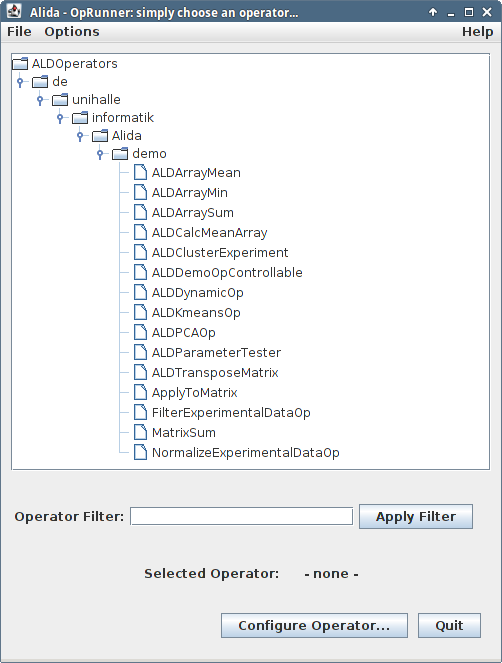
\includegraphics[width=0.425\textwidth]{../images/screenShotOpRunnerMain.png}
\caption{\label{fig:OpRunnerGUIMain}
	Screenshot of the main window of \alida's operator runner with the
	\icode{demo} package unfolded.}
\end{center}
\end{figure}

\begin{center}
\begin{figure}[t]
\begin{center}
\hspace*{4cm}
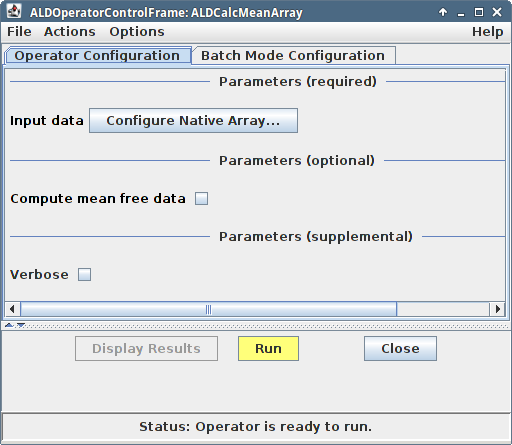
\includegraphics[width=0.55\textwidth,clip,trim=0 0 0 0]
				{../images/screenShotALDCalcMeanArray}\\[-1cm]
\hspace*{-3cm}
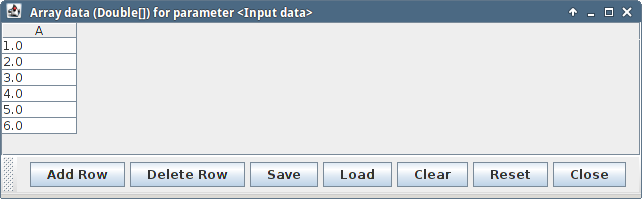
\includegraphics[width=0.7\textwidth,clip,trim=0 0 0 0]
				{../images/screenShotALDCalcMeanArrayConfig}\\
\caption{\label{fig:calcMeanArrayGUI}Screenshot of the automatically generated
control window for the operator {\tt ALDCalcMeanArray}.}
\end{center}
\end{figure}
\end{center}

\vspace*{-0.5cm}
The operator \icode{ALDCalcMeanArray} can also be invoked from command line,
without running the graphical user interface, via the application
\icode{ALDOpRunner}. It expects the values of all parameters being handed over
as command line argument strings. The operator can be executed as follows:
\vspace*{0.5cm}
\begin{code}
    java de.unihalle.informatik.Alida.tools.ALDOpRunner ALDCalcMeanArray \
        data='[1.0,1.5,2.2,0.4]' doMeanFree=true mean=- meanFreeData=-
\end{code}

\newpage
The call will execute the operator with a 1D array of four double values as
input data, and requests to compute the mean free data array in addition to the
mean of the data.
Setting the output parameters '\icode{mean}' and '\icode{meanFreeData}'
to~'\icode{-}' requests to print the results to the standard output, 
yielding the following output in the console:
\vspace*{0.5cm}
\begin{code}
  meanFreeData = [ -0.27500000000000013 , 0.22499999999999987 , 
                     0.925 , -0.8750000000000001 ]
  doMeanFree = true
  mean = 1.2750000000000001
\end{code}
\vspace*{-0.25cm}